% chapters/15/section-01.tex
\section{Mengapa Bunyi Penting}
\label{sec:peran-bunyi}

\subsection{Bunyi Menarik Perhatian dan Memperkuat Mekanik}

Sampai bab sebelumnya, seluruh umpan balik yang Anda pasang bersifat terlihat:
skor bertambah pada sudut layar, nyawa berkurang, animasi berganti. Umpan balik
yang terlihat saja tidak cukup, sebab pemain tidak selalu menatap bagian layar
yang berubah itu. Bunyi menjangkau pemain tanpa menuntut perhatian matanya,
sehingga ia menjadi jalan kedua untuk menyampaikan keadaan permainan
\cite{unity-leveldesign}.

Perhatikan Gambar~\ref{fig:petunjuk-visual-dan-bunyi}. Pada keadaan itu, pemain
hampir kehabisan persediaan udara. Keadaan itu disampaikan melalui tiga jalan
sekaligus: angka pada sudut kiri bawah, pesan tertulis di tengah layar, dan
bunyi yang berubah menjadi lebih mencekam.

\begin{figure}[htbp]
\centering
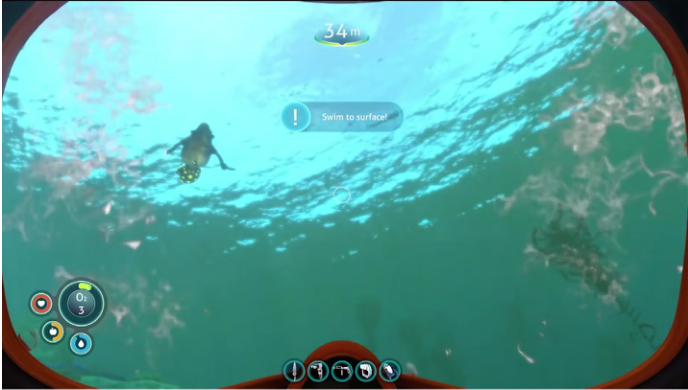
\includegraphics[width=0.78\textwidth]{figures/petunjuk-visual-dan-bunyi.png}
\caption{Peringatan yang disampaikan melalui tiga jalan sekaligus: angka, pesan tertulis, dan bunyi}
\label{fig:petunjuk-visual-dan-bunyi}
\sumber{[R12] halaman 35, dengan penyesuaian keterangan}
\end{figure}

Gambar itu memperlihatkan kebiasaan yang perlu Anda tiru. Setiap keterangan
yang disampaikan melalui bunyi sebaiknya disampaikan pula secara terlihat.
Pemain yang pendengarannya terganggu tetap dapat memahami keadaan permainan,
dan pemain lain memperoleh keterangan yang sama melalui dua jalan sekaligus.
Bunyi yang berdiri sendiri, tanpa pasangan yang terlihat, menutup permainan
bagi sebagian pemain, dan itu kerugian yang tidak perlu.

\begin{catatabox}
Pada Bab~XIV Anda menambahkan antarmuka yang menampilkan skor dan nyawa. Pada
bab ini, setiap bunyi diberi pasangan yang terlihat. Bunyi lompat berpasangan
dengan animasi lompatan, bunyi mengambil benda berpasangan dengan angka skor
yang bertambah, dan bunyi terluka berpasangan dengan nyawa yang berkurang.
\end{catatabox}

\subsection{Dua Jenis Bunyi dalam Permainan}

Tidak semua bunyi diperlakukan dengan cara yang sama. Ada dua jenis yang perlu
Anda bedakan sejak awal, dan perbedaannya menentukan cara memuat, memutar, dan
mengatur kekuatannya. Perbedaan itu dirangkum pada
Tabel~\ref{tab:bgm-sfx}.

\begin{table}[htbp]
\centering
\caption{Perbedaan musik latar dan efek suara}
\label{tab:bgm-sfx}
{\setlength{\tabcolsep}{4pt}\footnotesize%
\begin{tabularx}{\textwidth}{@{}L{2.6cm} Y Y@{}}
\toprule
\headrow \textbf{Segi} & \textbf{Musik latar (BGM)} & \textbf{Efek suara (SFX)} \\
\midrule
Lama berbunyi & Panjang, puluhan detik sampai beberapa menit & Pendek, umumnya di bawah dua detik \\
\addlinespace
Berapa kali & Satu berkas berjalan terus, diputar berulang & Banyak berkas pendek, dipanggil menurut kejadian \\
\addlinespace
Kapan dimulai & Ketika scene dimuat, bukan ketika sesuatu terjadi & Ketika peristiwa permainan terjadi \\
\addlinespace
Boleh bertumpuk & Tidak; musik baru menimpa musik lama & Ya; dua bunyi dapat berbunyi bersamaan \\
\addlinespace
Letak di ruang & Di mana-mana; tidak berubah oleh posisi pemain & Umumnya pada tempat kejadian, ikut melemah menurut jarak \\
\addlinespace
Kekuatan & Lebih pelan, sebab berjalan terus-menerus & Lebih kuat, sebab harus terdengar di atas musik \\
\bottomrule
\end{tabularx}}
\end{table}

Dua baris pada tabel itu perlu diperhatikan lebih saksama. Pertama, musik latar
tidak boleh bertumpuk. Apabila Anda memanggil bunyi musik dua kali, yang kedua
menimpa yang pertama, dan yang terdengar adalah keadaan yang tidak Anda
maksudkan. Kedua, efek suara justru perlu dapat bertumpuk. Pemain yang melompat
sambil mengambil benda menimbulkan dua bunyi dalam waktu yang sangat
berdekatan.

\begin{peringatanbox}
Kesalahan yang paling sering terjadi: memakai satu \code{AudioSource} untuk
musik dan efek suara sekaligus. Akibatnya, setiap efek suara menghentikan musik
yang sedang berjalan. Pisahkan keduanya sejak awal, misalnya menjadi
\code{musicSource} dan \code{sfxSource}, sebagaimana pada bab ini.
\end{peringatanbox}

Bunyi mana yang termasuk jenis yang mana ditentukan oleh keperluannya, bukan
oleh berkasnya. Berkas yang sama dapat dipakai sebagai musik latar pada satu
permainan dan sebagai efek suara pada permainan lain. Pertanyaan yang menuntun
pilihan Anda bukan ``berkas apa ini'', melainkan ``apakah bunyi ini berjalan
terus, atau dipanggil menurut kejadian''.
